\documentclass[11pt]{article}
\usepackage[T1]{fontenc}
\usepackage[utf8]{inputenc}
\usepackage{lmodern}
\usepackage[margin=1.05in]{geometry}
\usepackage{amsmath,amssymb,amsthm,mathtools}
\usepackage{booktabs,longtable,array}
\usepackage{microtype}
\usepackage{enumitem}
\usepackage{hyperref}
\usepackage{xcolor}
\usepackage{cleveref}
\usepackage{authblk}
\usepackage{mathrsfs}
\usepackage{graphicx}
\usepackage{tikz}
\usetikzlibrary{arrows.meta,calc}

\hypersetup{colorlinks=true,linkcolor=blue!55!black,citecolor=blue!55!black,urlcolor=blue!55!black}
\setlist{nosep}
\renewcommand{\arraystretch}{1.12}

\newtheorem{theorem}{Theorem}[section]
\newtheorem{proposition}[theorem]{Proposition}
\newtheorem{lemma}[theorem]{Lemma}
\newtheorem{corollary}[theorem]{Corollary}
\newtheorem{claim}[theorem]{Claim}
\theoremstyle{definition}
\newtheorem{definition}[theorem]{Definition}
\newtheorem{remark}[theorem]{Remark}
\newtheorem{example}[theorem]{Example}

\newcommand{\Z}{\mathbb Z}
\newcommand{\Tr}{\operatorname{Tr}}
\newcommand{\KH}{K_H}
\newcommand{\Kf}{K_{\mathrm{free}}}
\newcommand{\Gam}{\Gamma}
\newcommand{\eps}{\varepsilon}
\newcommand{\supp}{\operatorname{supp}}
\newcommand{\OO}{O}
\newcommand{\id}{\mathrm{id}}

\title{\textbf{Exterior-Turn Thresholds and Extremal Confinement Intensity\\for Exact-Trace Lattice Paths}}
\author[1]{Jorge Rosales P\'erez\thanks{ORCID: 0009-0008-1679-7858. Email: \texttt{mtro.jrp@gmail.com}.}}
\affil[1]{Independent Researcher, Mexico}
\date{External review draft v0.1 --- 24 August 2026}

\begin{document}
\maketitle

\begin{abstract}
Let $H=\{(x,y)\in\Z^2:y\ge0\}$ and let $U$ be a finite alphabet of primitive unoriented lattice directions.  For a finite trace $S\subset H$, write $K_H(S;U)$ for the minimum number of turns in a vertex-simple $U$-path whose vertex set is exactly $S$, and $K_{\rm free}(S;U)$ for the minimum number of turns in a $U$-path whose intersection with $H$ is exactly $S$, while the path may use vertices below the boundary.  Earlier work established that unbounded confinement gaps occur exactly when $U$ contains two nonparallel orientations.  Here we quantify the onset and extremal strength of that phenomenon.

We introduce the exterior-turn threshold
\[
\tau_H(U)=\min\Bigl\{k:\sup_{K_{\rm free}(S;U)\le k}K_H(S;U)=\infty\Bigr\}
\]
and the threshold intensity $\eta(U)$, the asymptotic density of the largest additive confinement gap at the threshold.  We prove that
\[
\tau_H(U)\in\{\infty,4,3,2\},
\]
and, whenever $\tau_H(U)<\infty$,
\[
\eta(U)\in\{1,2/3\}.
\]
Consequently the finite pairs are exactly
\[
(4,1),\ (3,1),\ (3,2/3),\ (2,1),\ (2,2/3).
\]
The proof combines a complete classification of residual pencil alphabets, rank-two determinant-multiplicity lemmas, single-rung extremal constructions, and a triangular-strip obstruction.  The delicate bounded-port triangular case is handled by an explicit 12-state connectivity-aware frontier automaton; its finite max-plus transfer relation gives a uniform $2/3$ turn-density bound while preserving boundary pairing.  Computations supplied with the manuscript are regression checks and finite certificates for displayed transition systems; no experimental search is used as a substitute for a universal argument.
\end{abstract}

\medskip
\noindent\textbf{Keywords.} lattice paths; minimum-link paths; Hamiltonian grid graphs; turn minimization; exact trace; computational geometry; discrete geometry; transfer matrices.

\section{Introduction}
A finite point set can be easy to visit if a path is allowed to leave the region in which the points live, yet expensive if every intermediate lattice vertex is required to remain in that region.  The distinction is especially sharp when paths are constrained to a finite direction alphabet and cost is measured in turns rather than Euclidean length.

We work in the fixed lattice half-plane
\[
H=\{(x,y)\in\Z^2:y\ge0\}.
\]
A path uses primitive lattice steps from a finite set $U$ of unoriented directions.  The trace is exact: every intermediate primitive lattice vertex of every long link counts.  Thus an exterior detour may save turns only if all of its additional lattice vertices lie outside $H$.

The qualitative starting point is the confinement theorem of \cite{RosalesPaperIIII}: unbounded gaps between the optimal confined and free turn counts exist if and only if $U$ contains at least two nonparallel orientations.  That theorem leaves two natural quantitative questions.

\begin{enumerate}[label=(Q\arabic*)]
\item How many turns must the free path be allowed before arbitrarily large confined complexity first becomes possible?
\item At that first budget, how large can the additive confinement gap be as a fraction of the trace size?
\end{enumerate}

The first question leads to $\tau_H(U)$; the second to an extremal gap function $\Gamma_U(k,N)$ and its threshold density $\eta(U)$.  The striking feature is that both parameters take only a small number of values.

\subsection{Main results}
Our first theorem classifies the onset threshold.

\begin{theorem}[Global threshold classification]\label{thm:global-tau}
Let $U$ be a finite set of primitive unoriented lattice directions.  Then
\[
\boxed{\tau_H(U)\in\{\infty,4,3,2\}.}
\]
The value $\infty$ occurs for a one-orientation alphabet.  In the residual pencil coordinates
\[
U_J=\{(1,0),(0,1)\}\cup\{(1,k):k\in J\},\qquad J\subset\Z_{>0}\text{ finite},
\]
one has
\[
\boxed{
\tau_H(U_J)=
\begin{cases}
4,&J=\varnothing,\\
3,&J=\{1\}\text{ or }\{1,2\},\\
2,&\text{otherwise}.
\end{cases}}
\]
All non-pencil determinant-generic alphabets have threshold $2$.
\end{theorem}

The threshold is a genuine phase transition for the extremal gap.

\begin{theorem}[Bounded-to-linear transition]\label{thm:Gamma-jump}
For fixed $U$ and integer $k\ge0$, define
\[
\Gamma_U(k,N)=\max\{K_H(S;U)-K_{\rm free}(S;U): S\text{ admissible},\ |S|\le N,\ K_{\rm free}(S;U)\le k\}.
\]
If $\tau_H(U)<\infty$, then
\[
\boxed{
 k<\tau_H(U)\Longrightarrow \Gamma_U(k,N)=O_{U,k}(1),
 \qquad
 k\ge\tau_H(U)\Longrightarrow \Gamma_U(k,N)=\Theta_U(N).}
\]
\end{theorem}

At onset there are exactly two asymptotic intensities.

\begin{theorem}[Global threshold-intensity classification]\label{thm:global-eta}
For finite threshold define
\[
\eta(U)=\limsup_{N\to\infty}\frac{\Gamma_U(\tau_H(U),N)}{N}.
\]
Then
\[
\boxed{\eta(U)\in\{1,2/3\}.}
\]
Hence the complete set of finite pairs is
\[
\boxed{(\tau_H(U),\eta(U))\in
\{(4,1),(3,1),(3,2/3),(2,1),(2,2/3)\}.}
\]
\end{theorem}

The two intensities correspond to two different induced-graph mechanisms.  A \emph{single-rung} rail pair can force almost every internal Hamiltonian vertex to turn, giving density $1$.  A determinant-balanced pair of adjacent rails carries two interlaced rung families and forms a triangular strip.  The second rung family creates unavoidable straight-through opportunities and lowers the sharp density to $2/3$.

\subsection{Proof architecture}
The proof has four layers.

First, the qualitative dichotomy of \cite{RosalesPaperIIII} reduces the only nongeneric case to a residual pencil.  We classify all pencils and prove that the exceptional alphabets $U_{\{1\}}$ and $U_{\{1,2\}}$ really have threshold $3$ by an explicit boundary-entry bridge lemma.

Second, we prove extremal single-rung families with $K_H=|S|-O_U(1)$ in every intensity-one branch.

Third, we study determinant multiplicities.  A finite primitive direction set with at least four directions always has a singleton transverse determinant class unless it is the special balanced triple.  With at least five directions a singleton can be chosen away from any prescribed direction, in particular away from the horizontal.  Such a nonhorizontal singleton produces a single-rung family at budget two.

Finally, the balanced residual case is triangular.  The canonical fixed-terminal strip has an exact four-state calculation.  Arbitrary bounded-port replacement requires more information: a cut state must remember not only which edges cross but also which crossing stubs are connected through the processed prefix.  An explicit 12-state connectivity automaton gives the uniform bound needed for both the unit-triangular four-link case and the nondivisible balanced four-direction residual.

\section{Model and notation}\label{sec:model}
\begin{definition}[Direction alphabet and path]
A \emph{direction} is an unoriented primitive lattice class $\{u,-u\}$ with $u\in\Z^2$ primitive.  A finite alphabet $U$ is a finite set of such classes.  A $U$-path $P=(p_0,\ldots,p_m)$ is vertex-simple and every increment $p_{i+1}-p_i$ is one primitive step in a class from $U$.
\end{definition}

A \emph{link} is a maximal consecutive run of steps having the same unoriented direction.  If $L(P)$ is the number of links, then
\[
K(P)=L(P)-1
\]
is the turn count.  Compressed long segments are merely notation: they are always expanded into primitive steps before traces are evaluated.

\begin{definition}[Exact host trace]
For a path $P$, define
\[
\Tr_H(P)=V(P)\cap H.
\]
For finite $S\subset H$ put
\[
K_H(S;U)=\min\{K(P):P\text{ is a $U$-path and }V(P)=S\},
\]
\[
K_{\rm free}(S;U)=\min\{K(P):P\text{ is a $U$-path and }\Tr_H(P)=S\}.
\]
The minimum of the empty set is $\infty$.  The trace $S$ is \emph{admissible} if both minima are finite.
\end{definition}

The induced confined graph $G_U(S)$ has vertex set $S$ and a primitive edge $pq$ whenever $q-p$ is one step in an allowed direction.  A confined exact path is therefore a Hamiltonian path of $G_U(S)$, with a direction label on each edge and turn cost on consecutive labels.

\begin{definition}[Threshold and extremal functions]
The exterior-turn threshold is
\[
\tau_H(U)=\min\Bigl\{k\ge0:\sup_{\substack{S\text{ admissible}\\K_{\rm free}(S;U)\le k}}K_H(S;U)=\infty\Bigr\},
\]
with value $\infty$ when the set is empty.  Define
\[
\Delta_H(S;U)=K_H(S;U)-K_{\rm free}(S;U),
\]
\[
\Gamma_U(k,N)=\max\{\Delta_H(S;U):S\text{ admissible},\ |S|\le N,\ K_{\rm free}(S;U)\le k\},
\]
and
\[
\gamma_U(k)=\limsup_{N\to\infty}\frac{\Gamma_U(k,N)}{N}.
\]
When $\tau_H(U)<\infty$, set $\eta(U)=\gamma_U(\tau_H(U))$.
\end{definition}

Every Hamiltonian path on $n$ vertices has at most $n-2$ turns, so $0\le\gamma_U(k)\le1$.

\section{Two elementary support lemmas}\label{sec:support}
The following counting observation recurs throughout the paper.

\begin{lemma}[Nonparallel support sparsity]\label{lem:support-sparsity}
Let $L,M$ be two nonparallel lattice lines.  For a fixed finite alphabet $U$, the number of primitive allowed edges having one endpoint on $L$ and one on $M$ is at most $2|U|$.
\end{lemma}
\begin{proof}
Fix a signed primitive representative $s$ of an allowed direction.  If $x\in L$ and $x+s\in M$, then
\[
x\in L\cap(M-s).
\]
Because $L$ and $M-s$ are nonparallel, this intersection contains at most one point.  Sum over the two signs of each direction in $U$.
\end{proof}

\begin{lemma}[One-turn obstruction]\label{lem:one-turn}
For every fixed finite alphabet $U$,
\[
K_{\rm free}(S;U)\le1\Longrightarrow K_H(S;U)=O_U(1).
\]
Consequently every finite threshold satisfies $\tau_H(U)\ge2$.
\end{lemma}
\begin{proof}
A free path with at most one turn lies on one or two support lines.  If there is one support, the confined trace is a single interval and has zero turns.  If there are two nonparallel supports, \cref{lem:support-sparsity} gives $O_U(1)$ inter-support edges.  Along either support every used rail edge is straight, so every turn of a Hamiltonian path, except for a constant number at the support intersection and endpoints, is incident to an inter-support edge.  Hence the confined turn count is uniformly bounded.
\end{proof}

\section{The rectilinear threshold}\label{sec:rect}
Let $U_\square=\{(1,0),(0,1)\}$.

\begin{proposition}[Rectilinear low-turn rigidity]\label{prop:rect-rigidity}
For every admissible $S\subset H$,
\[
K_{\rm free}(S;U_\square)\le3\Longrightarrow K_H(S;U_\square)=K_{\rm free}(S;U_\square).
\]
\end{proposition}
\begin{proof}
Choose an optimal free path and remove any wholly exterior prefix and suffix.  If the host vertices are consecutive along the path, clipping between the first and last host vertex already gives a confined path with no larger turn count.

Otherwise the path leaves $H$ and later re-enters.  With at most four rectilinear links, up to reversal the nontrivial forms are
\[
V-H_{\rm out}-V
\quad\text{or}\quad
H-V-H_{\rm out}-V.
\]
In the first form the trace is two vertical columns.  Admissibility forces the columns to be horizontally adjacent; moving the exterior horizontal link to $y=0$ gives a confined path with at most two turns.

For the second form, after reflection write the compressed path as
\[
(c,A)\to(a,A)\to(a,-d)\to(b,-d)\to(b,B),\qquad a<c.
\]
The trace consists of the horizontal arm
\[
R=\{(x,A):a\le x\le c\}
\]
and columns $C_a,C_b$.  Since the path is vertex-simple, $C_b\cap R=\varnothing$.  If the induced grid graph is connected, exactly one of the following occurs:
\begin{enumerate}[label=(\roman*)]
\item $|a-b|=1$;
\item $a<b\le c$ and $B=A-1$;
\item $b=c+1$ and $B\ge A$.
\end{enumerate}
Indeed, after excluding direct column-column adjacency, any contact from $C_b$ to $R$ is vertical or horizontal.

In (i) move the exterior link to $y=0$.  In (ii), if $a<b<c$, the induced graph has three leaves $(a,0),(b,0),(c,A)$ and cannot have a Hamiltonian path; hence $b=c$, where a two-turn traversal exists.  In (iii), if $A>0$ and $B>A$, the vertices $(a,0),(b,0),(b,B)$ are three leaves; hence $B=A$ and again a two-turn traversal exists.  The degeneracy $A=0$ is simpler.  Thus every admissible trace produced with at most three free turns clips without increasing the turn count.
\end{proof}

\begin{proposition}[Sharp rectilinear ladder]\label{prop:rect-ladder}
For even $t\ge2$, let
\[
S_t^*=\{(i,1):0\le i\le t\}\cup\{(i,2):1\le i\le t\}\cup\{(0,0),(t,0)\}.
\]
Then
\[
|S_t^*|=2t+3,\qquad K_{\rm free}(S_t^*;U_\square)=4,
\]
and
\[
K_H(S_t^*;U_\square)=2t=|S_t^*|-3.
\]
\end{proposition}
\begin{proof}
The compressed free witness
\[
(t-1,1)\to(0,1)\to(0,-1)\to(t,-1)\to(t,2)\to(1,2)
\]
has four turns and, after primitive expansion, exact host trace $S_t^*$.  In $G_{U_\square}(S_t^*)$, the two bottom vertices force the Hamiltonian endpoints and degree propagation determines the Hamiltonian order up to reversal.  Exactly one internal vertex is straight, so $K_H=|S|-3$.  By \cref{prop:rect-rigidity}, the free cost cannot be at most three, hence it is exactly four.
\end{proof}

\begin{corollary}\label{cor:rect-tau-eta}
\[
\boxed{\tau_H(U_\square)=4,\qquad \eta(U_\square)=1.}
\]
\end{corollary}

\section{Residual pencils and the complete threshold classification}\label{sec:pencils}
We use the qualitative determinant dichotomy from \cite{RosalesPaperIIII}.  Its residual case can be expressed inside a lattice coset using a horizontal primitive direction $h$ and a nonhorizontal primitive direction $v$.

\begin{lemma}[Coset normalization]\label{lem:coset}
Let $L=\Z h+\Z v$ and let a path lie in a coset $c+L$.  Choose the representative $c$ with $0\le c_y<v_y$.  Then
\[
\Psi_c(i,j)=c+ih+jv
\]
is injective, maps $j\ge0$ exactly to $H\cap(c+L)$, and preserves primitive adjacency, vertex simplicity, exact host trace, links and turns.  Consequently residual threshold questions reduce exactly to
\[
U_J=\{h=(1,0),v=(0,1)\}\cup\{d_k=(1,k):k\in J\}.
\]
\end{lemma}
\begin{proof}
Injectivity follows from linear independence.  By the chosen representative, $(\Psi_c(i,j))_y=c_y+jv_y\ge0$ if and only if $j\ge0$.  Every allowed primitive step in the coset corresponds to one allowed coordinate step and conversely; all remaining assertions follow immediately.
\end{proof}

\subsection{The two exceptional nonrectilinear pencils}
Write $U_1=U_{\{1\}}$ and $U_{12}=U_{\{1,2\}}$.

\begin{lemma}[Boundary-entry bridge]\label{lem:bridge}
Consider a free path with at most two turns whose first and third support lines are parallel in direction $r$, with middle direction $q$.  Suppose a direct primitive allowed edge $w$ joins the two rails.  If the middle link has $\ell$ primitive $q$-steps, then
\[
|\det(r,w)|=\ell|\det(r,q)|.
\]
For $U_1$, every nonhorizontal case has $\ell=1$.  For $U_{12}$, every nonhorizontal case has $\ell\le2$.  Moreover, in every determinant-permitted case the first host vertices on the two rails are joined by one permitted primitive edge; if $\ell=2$, the middle connector has at most one visible internal vertex, which can be inserted by a constant-size splice.
\end{lemma}
\begin{proof}
The determinant identity follows because the rail separation equals $\ell q+kr$ for some integer $k$; taking determinant with $r$ removes the $kr$ term.

For $U_1$, all nonzero pairwise determinant magnitudes are $1$, hence $\ell=1$.  For $U_{12}=\{h,v,d_1,d_2\}$ the only determinant magnitude larger than $1$ is $|\det(d_2,h)|=2$, hence $\ell\le2$.

It remains to verify the boundary entries.  Orient $r_y>0$.  If the first host height on one rail has residue $s\in\{0,\ldots,r_y-1\}$, the first host height on the translated rail is the residue
\[
s'\equiv s+\ell q_y\pmod{r_y}.
\]
Their difference is
\[
\ell q+kr,
\qquad k=\frac{s'-(s+\ell q_y)}{r_y}.
\]
The finitely many possible triples $(r,q,\ell)$ and residues are displayed in \cref{tab:bridge-summary,tab:bridge-full}.  In every nonhorizontal row this difference is one primitive allowed direction.  Horizontal rails clip directly.  When $\ell=2$, only one connector vertex can lie strictly between the two rail supports, so it changes the splice by a constant number of turns.
\end{proof}

\begin{table}[t]
\centering
\caption{Boundary-entry bridge summary.  The full residue table is in \cref{tab:bridge-full}.}
\label{tab:bridge-summary}
\begin{tabular}{lll}
\toprule
Alphabet & possible connector length & conclusion\\
\midrule
$U_1$ & $\ell=1$ & first host rail entries are primitively adjacent\\
$U_{12}$ & $\ell=1,2$ & first host rail entries are primitively adjacent\\
\bottomrule
\end{tabular}
\end{table}

\begin{proposition}[Exceptional thresholds]\label{prop:exceptional-thresholds}
\[
\boxed{\tau_H(U_1)=3,\qquad \tau_H(U_{12})=3.}
\]
\end{proposition}
\begin{proof}
For the lower bound, let a free witness have at most two turns.  If its host vertices are consecutive, clip it.  Otherwise the trace lies on at most three supports.  If the outer supports are nonparallel, \cref{lem:support-sparsity} bounds all changes of support.  If the outer supports are parallel but no direct rail edge exists, all transitions use the middle support and are again bounded.  If a rail edge exists, \cref{lem:bridge} replaces the possibly split boundary entry by a constant-size confined splice.  Hence $K_H=O(1)$ for every trace with $K_{\rm free}\le2$.

For the upper bound, explicit three-turn families exist.  For $U_1$, take
\[
A_i=(0,i),\ 0\le i\le n,
\qquad B_j=(1,j),\ 1\le j\le n+2,
\]
plus $C_0=(2,0),C_1=(2,1),D=(3,1)$.  The free witness
\[
(0,n)\to(0,-2)\to(3,1)\to(1,1)\to(1,n+2)
\]
has directions $v,d_1,h,v$ and exact declared trace.  The two-rail core has only bounded cross shifts and the terminal gadget forces endpoints, so the two-rail cut lemma of \cite{RosalesPaperIIII} gives $K_H\to\infty$.  The $U_{12}$ construction is analogous; its threshold-three single-rung family is given explicitly in \cref{prop:u12-extremal}.
\end{proof}

\subsection{All remaining pencils have threshold two}
\begin{proposition}[Top-gap family]\label{prop:top-gap}
Let $J\ne\varnothing$, $K=\max J$, $a=\max(\{0\}\cup(J\setminus\{K\}))$, and $g=K-a$.  If $g\ge2$, then $\tau_H(U_J)=2$.
\end{proposition}
\begin{proof}
Put $r=g-1$ and, for even $p$, define
\[
A_i=(i,r+Ki),\quad0\le i\le p,
\]
\[
B_j=(j,-1+Kj),\quad1\le j\le p,
\]
and $C_y=(0,y)$ for $0\le y<r$.  The compressed free witness
\[
A_p\to A_0\to(0,-1)\to B_p
\]
has two turns.  Its vertical middle link visits the entire cap before leaving $H$, so the exact trace is the declared set.

For $m=j-i$,
\[
B_j-A_i=(m,Km-g).
\]
The only primitive cross edge occurs for $m=1$, giving $(1,a)$.  The two leaves force Hamiltonian endpoints, and degree propagation gives $K_H=2p$; the cap contributes only a constant straight prefix.  Thus the confined cost is linear while the free cost is two.  The one-turn obstruction gives equality of the threshold.
\end{proof}

\begin{proposition}[Consecutive-block family]\label{prop:consecutive}
If
\[
m\ge2,\qquad m,m+1\in J,\qquad m-1\notin J,
\]
then $\tau_H(U_J)=2$.
\end{proposition}
\begin{proof}
Set
\[
B_i=(i,mi),\qquad A_i=(i+1,mi+m-1),\qquad0\le i\le p.
\]
The free witness $A_p\to A_{-2}\to B_{-1}\to B_p$ has two turns and exact two-rail trace, since its middle vertical edge is below $H$.  For $k=j-i$,
\[
B_j-A_i=(k-1,m(k-1)+1).
\]
The determinant-permitted primitive cross shifts are exactly $k=1,2$: $k=0$ would be $d_{m-1}$, which is absent.  The endpoints $B_0,A_p$ are leaves, and the Hamiltonian path
\[
B_0,B_1,A_0,B_2,A_1,\ldots,B_p,A_{p-1},A_p
\]
shows admissibility.  The two-rail cut lemma forces linearly many rail changes and hence turns.
\end{proof}

\begin{proposition}[Full initial blocks]\label{prop:initial-block}
If $J=\{1,2,\ldots,K\}$ with $K\ge3$, then $\tau_H(U_J)=2$.
\end{proposition}
\begin{proof}
Let $g=K-1$ and define
\[
A_i=(i,i),\quad0\le i\le p,
\qquad
B_j=(j,j-g),\quad g\le j\le p-2.
\]
The free witness
\[
A_p\to A_{-1}\to B_{-1}\to B_{p-2}
\]
has two turns and its middle vertical connector is entirely below $H$.  For $m=j-i$,
\[
B_j-A_i=(m,m-g).
\]
The only primitive cross family in the trace is $m=-1$, corresponding to $d_K$.  A forced finite $A$-prefix is followed by a parity-controlled alternating Hamiltonian core.  In particular $K_H=\Theta(p)$ while $|S|=\Theta(p)$.
\end{proof}

\begin{lemma}[Pencil exhaustion]\label{lem:pencil-exhaust}
Every finite $J\subset\Z_{>0}$ other than $\varnothing,\{1\},\{1,2\}$ satisfies one of \cref{prop:top-gap,prop:consecutive,prop:initial-block}.
\end{lemma}
\begin{proof}
Let $K=\max J$ and let $a$ be the next largest element, or $0$.  If $K-a\ge2$, use the top-gap case.  Otherwise $K-1\in J$.  Descend from $K$.  If the descent first stops at some $m\ge2$, then $m,m+1\in J$ while $m-1\notin J$, giving the consecutive-block case.  If it never stops before $1$, then $J=\{1,\ldots,K\}$; excluding $\{1\}$ and $\{1,2\}$ leaves $K\ge3$.
\end{proof}

\begin{proof}[Proof of \cref{thm:global-tau}]
A one-orientation alphabet has no turns and therefore threshold $\infty$.  If $U$ has at least two nonparallel orientations, the qualitative theorem of \cite{RosalesPaperIIII} gives a dichotomy.  In the determinant-generic branch, its explicit two-turn amplifier together with \cref{lem:one-turn} gives threshold $2$.  The residual branch is a pencil after \cref{lem:coset}.  The rectilinear case is \cref{cor:rect-tau-eta}; the two exceptional pencils are \cref{prop:exceptional-thresholds}; every other pencil has threshold $2$ by \cref{lem:pencil-exhaust}.  No other values occur.
\end{proof}

\section{The extremal transition and intensity-one mechanisms}\label{sec:extremal}
\begin{proof}[Proof of \cref{thm:Gamma-jump}]
If $k<\tau_H(U)$, then by definition $K_H$ is uniformly bounded on all traces with $K_{\rm free}\le k$.  Since $0\le\Delta_H\le K_H$, the same is true of $\Gamma_U(k,N)$.

At and above threshold, the constructions used in the classification can be chosen with a parameter $p$ such that
\[
|S_p|=O_U(p),\qquad K_{\rm free}(S_p;U)\le\tau_H(U),\qquad K_H(S_p;U)=\Omega_U(p).
\]
Hence $\Gamma_U(k,N)=\Omega_U(N)$ for $k\ge\tau_H(U)$.  The universal Hamiltonian bound $K_H\le |S|-2\le N-2$ gives $O(N)$.
\end{proof}

We next record the families that reach intensity one.

\begin{proposition}[A uniform single-rung family]\label{prop:single-rung-pencil}
For $m\ge2$, let
\[
U_{m,m+1}=\{(1,0),(0,1),(1,m),(1,m+1)\}.
\]
There are traces $S_p$ with
\[
K_{\rm free}(S_p;U_{m,m+1})=2,
\qquad
K_H(S_p;U_{m,m+1})=|S_p|-2.
\]
\end{proposition}
\begin{proof}
Set $K=m+1$, $C=(0,0)$,
\[
A_i=(i,Ki+1),\quad0\le i\le p,
\qquad
B_j=(j,Kj-K+1),\quad1\le j\le p,
\]
with $p$ even.  The free witness
\[
A_p\to A_0\to(0,1-K)\to B_p
\]
has two turns and exact trace $S_p=\{C\}\cup\{A_i\}\cup\{B_j\}$.  Since $d_1$ is absent, $C$ is a leaf.  For opposite rails, the only primitive cross family is the horizontal rung $A_iB_{i+1}$.  The opposite extreme is also a leaf.  Degree propagation forces the unique Hamiltonian path up to reversal, and every internal vertex turns.  Thus $K_H=|S|-2$.  The one-turn obstruction gives $K_{\rm free}=2$.
\end{proof}

\begin{proposition}[$U_{12}$ at threshold three]\label{prop:u12-extremal}
For $U_{12}=\{h,v,d_1,d_2\}$ there are traces $S_p$ with
\[
K_{\rm free}(S_p;U_{12})=3,
\qquad
K_H(S_p;U_{12})=|S_p|-2.
\]
Hence $\eta(U_{12})=1$.
\end{proposition}
\begin{proof}
For even $p$, let
\[
A_i=(i,2i+1),\quad0\le i\le p,
\qquad B_j=(j-2,2j-1),\quad1\le j\le p,
\]
and $C=(0,0)$.  The free witness
\[
A_p\to A_0\to(0,-1)\to(-2,-1)\to B_p
\]
has directions $d_2,v,h,d_2$ and three turns.  For $k=j-i$,
\[
B_j-A_i=(k-2,2k-2),
\]
and only $k=1$ gives a primitive allowed cross edge, a horizontal rung.  The cap and opposite extreme force the endpoints; every internal Hamiltonian vertex turns.  Thus $K_H=|S|-2$.  By \cref{prop:exceptional-thresholds}, the free cost cannot be at most two for sufficiently large members, so it equals three.
\end{proof}

\begin{proposition}[Pencil intensity]\label{prop:pencil-intensity}
For every finite pencil $U_J$,
\[
(\tau_H(U_J),\eta(U_J))=
\begin{cases}
(4,1),&J=\varnothing,\\
(3,2/3),&J=\{1\},\\
(3,1),&J=\{1,2\},\\
(2,1),&\text{otherwise}.
\end{cases}
\]
The unit-triangular value $2/3$ is proved in \cref{sec:triangular}.
\end{proposition}
\begin{proof}
The first and third lines are \cref{cor:rect-tau-eta,prop:u12-extremal}.  If $1\notin J$, use the maximal slope $d_K$ in the construction of \cref{prop:single-rung-pencil}; the missing $d_1$ leaves only a horizontal rung family and gives $K_H=|S|-O_J(1)$.  If $1\in J$ and $K=\max J\ge3$, take $g=K-1$ and the $d_1$-rail family of \cref{prop:initial-block}.  A direct degree count gives
\[
K_H=|S|-g-2=|S|-K-1,
\]
so the threshold gap density tends to one.
\end{proof}

\section{Determinant multiplicity}\label{sec:determinant}
For $r\in U$ and $\delta>0$ define
\[
m_r(\delta)=\#\{w\in U\setminus\{r\}:|\det(r,w)|=\delta\}.
\]
A value with multiplicity one is a \emph{singleton transverse determinant class}.

\begin{lemma}[Balanced triple algebra]\label{lem:balanced-algebra}
Suppose $u,v,w$ are pairwise nonparallel primitive directions and
\[
|\det(u,v)|=|\det(v,w)|=|\det(w,u)|=D>0.
\]
After sign choices,
\[
\boxed{w=u+v.}
\]
\end{lemma}
\begin{proof}
Choose signs so that $\det(u,v)=\det(u,w)=D$.  Then $\det(u,w-v)=0$, so by primitivity $w-v=ku$ for some integer $k$.  Taking determinant with $v$ gives $|k|D=D$, hence $|k|=1$; reverse a sign if necessary.
\end{proof}

\begin{lemma}[Hexagonal determinant contraction]\label{lem:hex-contraction}
Let $T=\{u,v,u+v\}$ with $|\det(u,v)|=M$.  Write $z=au+bv$ and $x=cu+dv$ in the real span and set
\[
\rho(a,b)=\max\{|a|,|b|,|a-b|\}.
\]
Then
\[
\max_{t\in T}|\det(z,t)|=M\rho(a,b)
\]
and
\[
|\det(z,x)|\le M\rho(a,b)\rho(c,d).
\]
\end{lemma}
\begin{proof}
The three determinants are $M|b|,M|a|,M|a-b|$.  The second inequality is the standard determinant estimate for the hexagonal norm; by homogeneity it suffices to check it on the six vertices of the unit hexagon $\rho\le1$, where it is immediate.
\end{proof}

\begin{theorem}[Singleton Determinant Theorem]\label{thm:singleton}
If $U$ is a finite set of distinct primitive unoriented lattice directions with $|U|\ge4$, then
\[
\boxed{\exists r\in U,\ \delta>0:\ m_r(\delta)=1.}
\]
More precisely, among nontrivial alphabets the only sets with no singleton determinant class are determinant-balanced triples.
\end{theorem}
\begin{proof}
Assume that no singleton class exists.  Let
\[
M=\max_{x\ne y\in U}|\det(x,y)|
\]
and choose $u,v$ attaining $M$.  Since the value $M$ is not singleton in row $u$, there is $w\ne v$ with $|\det(u,w)|=M$.  Choose signs with $\det(u,v)=\det(u,w)=M$.  Then $w-v=ku$; maximality gives $|\det(v,w)|=|k|M\le M$, while $k\ne0$, so $|k|=1$.  Thus $T=\{u,v,u+v\}$ is a balanced triangle.

No external direction can be joined by a determinant-$M$ edge to a member of $T$: if, for example, $|\det(u,z)|=M$, the same preceding argument applied to $u$ and its two $M$-neighbors forces $z$ to be the third direction of the same balanced triangle.  Hence every $z\in U\setminus T$ has
\[
D(z):=\max_{t\in T}|\det(z,t)|<M.
\]
For an external primitive direction the maximum among the three values in $D(z)$ is unique.  Indeed, a tie in the hexagonal norm $\rho$ lies on one of the three lines parallel to $u$, $v$, or $u+v$; primitivity and unoriented distinctness would then make $z$ one of the directions in $T$.

Choose external $z$ maximizing $D(z)$.  If the unique value $D(z)$ in row $z$ is not a singleton, some external $x$ must repeat it.  By \cref{lem:hex-contraction},
\[
|\det(z,x)|\le\frac{D(z)D(x)}{M}\le\frac{D(z)^2}{M}<D(z),
\]
a contradiction.  Therefore no external $z$ exists and $U=T$.  The converse is immediate: every determinant value in a balanced triple occurs twice in each row.
\end{proof}

\subsection{Singletons and intensity one}
\begin{proposition}[Nonhorizontal singleton bridge]\label{prop:nonhorizontal-singleton}
Suppose $r,q\in U$ are nonparallel, both have nonzero vertical coordinate, and
\[
m_r(|\det(r,q)|)=1.
\]
Then
\[
\boxed{(\tau_H(U),\eta(U))=(2,1).}
\]
\end{proposition}
\begin{proof}
Orient $r_y,q_y>0$ and put $d=\lceil q_y/r_y\rceil$.  For $p>d$ with $p-d$ even, set
\[
A_i=ir,\quad0\le i\le p,
\qquad
B_j=jr-q,\quad d\le j\le p-1.
\]
The compressed path
\[
A_p\to A_{-1}\to B_{-1}\to B_{p-1}
\]
has directions $r,q,r$ and two turns.  Its exact host trace is the displayed union, because $A_{-1}$ and $B_{-1}$ lie below $H$, while $B_j\in H$ exactly for $j\ge d$.

For a cross edge,
\[
B_j-A_i=(j-i)r-q
\]
has determinant magnitude $|\det(r,q)|$ with $r$.  By the singleton hypothesis the only permitted transverse direction in that determinant class is $q$, so the only cross edges are $A_iB_i$.  The resulting graph is a single-rung ladder with a forced straight prefix of length $O_U(1)$ and an alternating core in which every remaining internal vertex turns.  In fact
\[
K_H=2(p-d)=|S|-d-1.
\]
Thus $K_H/|S|\to1$.  The one-turn obstruction gives $\tau=2$.
\end{proof}

\subsection{A singleton away from any prescribed direction}
\begin{lemma}[Primitive-sum parity]\label{lem:parity}
If $a,b,a+b$ are primitive lattice vectors, then $\det(a,b)$ is odd.
\end{lemma}
\begin{proof}
Modulo $2$, primitive vectors are nonzero.  If $\det(a,b)$ were even, $a$ and $b$ would be dependent in $\mathbb F_2^2$, hence equal; then $a+b\equiv0\pmod2$, contradicting primitivity.
\end{proof}

\begin{theorem}[Distinguished Singleton Theorem]\label{thm:distinguished}
Let $U$ be a finite primitive direction set with $|U|\ge5$, and fix $e\in U$.  Then there exist $r,q\in U\setminus\{e\}$ such that
\[
\boxed{m_r(|\det(r,q)|)=1.}
\]
\end{theorem}
\begin{proof}
Let $M$ be the maximum determinant magnitude and let $G_M$ join two directions when their determinant magnitude is $M$.  Repetition of a maximum in a row and \cref{lem:balanced-algebra} show that every nontrivial component of $G_M$ is either a single edge or a balanced triangle.

A single edge avoiding $e$ already gives the conclusion.  A balanced triangle avoiding $e$ also gives the conclusion unless $U$ is exactly that triangle, by the contraction argument in \cref{thm:singleton}; here $|U|\ge5$.  If a maximal balanced triangle contains $e$, normalize it as
\[
e=(1,0),\qquad u=(a,M),\qquad v=(a+1,M).
\]
For any exterior upper representative $z=(p,y)$ with $0<y<M$, absence of an $e$-avoiding singleton forces $e$ to be the unique maximum neighbor of $z$.  Writing
\[
A_z=pM-ay,
\]
one obtains $0<A_z<y$.  The values $A_z$ are distinct because $\gcd(a,M)=1$; hence row $u$ acquires an $e$-avoiding singleton, a contradiction.

The only residual possibility is that $G_M$ consists of one edge $e-r$.  If no $e$-avoiding singleton exists, every nonzero determinant class in row $r$ must occur in a pair.  The determinant equation has at most two representatives for a fixed class, so
\[
U=\{e,r\}\cup\bigcup_i\{x_i,r-x_i\}.
\]
This is the paired-star form.  By \cref{lem:parity}, every
\[
d_i=|\det(r,x_i)|
\]
is odd.  Choose a largest class $D$ and a smaller class $d$.  Let $x$ lie in the $D$-pair and $y,r-y$ in the $d$-pair.  If a non-$e$ direction $z$ repeats $\alpha=|\det(x,y)|$, then after signs $z=\pm y+kx$ and
\[
\det(r,z)=\pm d+kD.
\]
The cases $|k|\ge2$ exceed $D$; $k=0$ gives the same direction; and $k=\pm1$ gives either $D+d>D$ or the positive even value $D-d$, impossible because all paired-star classes are odd.  Thus $\alpha$ has no non-$e$ repeater.  The same argument applies to $\beta=|\det(x,r-y)|$, and $\alpha\ne\beta$.  The distinguished direction $e$ can duplicate at most one of these two values in row $x$, so the other is an $e$-avoiding singleton.
\end{proof}

\begin{corollary}\label{cor:large-U}
If $|U|\ge5$, then
\[
\boxed{(\tau_H(U),\eta(U))=(2,1).}
\]
\end{corollary}
\begin{proof}
If $U$ contains a horizontal direction, apply \cref{thm:distinguished} with that direction as $e$; otherwise choose arbitrary $e$.  The resulting singleton pair is nonhorizontal, so \cref{prop:nonhorizontal-singleton} applies.
\end{proof}

\section{The triangular mechanism}\label{sec:triangular}
The only obstruction to intensity one is the determinant-balanced triangular mechanism.  We begin with a canonical strip.

\subsection{The fixed-terminal canonical strip}
Let $T_n$ have vertices
\[
A_0,\ldots,A_n,\qquad B_0,\ldots,B_{n+1},
\]
rail edges $A_iA_{i+1}$ and $B_jB_{j+1}$, and cross edges
\[
A_iB_i,\qquad A_iB_{i+1}.
\]
Fix Hamiltonian endpoints $B_0$ and $B_{n+1}$.

\begin{theorem}[Terminal-constrained strip theorem]\label{thm:terminal-strip}
For the preceding endpoint-constrained problem,
\[
\boxed{K_H^{\rm term}(T_n)=\left\lfloor\frac{2|V(T_n)|}{3}\right\rfloor.}
\]
\end{theorem}
\begin{proof}
For cut $i$, let $a_i,b_i$ indicate whether rail edges $A_iA_{i+1}$ and $B_iB_{i+1}$ are used, and let $c_i$ indicate the diagonal $A_iB_{i+1}$.  Cut parity for a Hamiltonian path with the prescribed endpoints gives
\[
a_i+b_i+c_i\equiv1\pmod2,
\]
so $c_i=1$ exactly when $a_i=b_i$.  Degree two at the two vertices of the next column yields the four-state transition system
\[
\begin{array}{c|l}
00&00,10,11\\
01&00,10,11\\
10&01\\
11&00,10.
\end{array}
\]
A straight vertex is earned only on
\[
01\to11\qquad\text{or}\qquad11\to10.
\]
The allowed initial states are $00,10,11$ and the terminal states are $00,01$.  A direct max-plus induction gives the largest possible number of straight internal vertices
\[
s_n=\left\lfloor\frac{2n-1}{3}\right\rfloor.
\]
Since $|V(T_n)|=2n+3$, every other internal vertex turns and
\[
K_H^{\rm term}=2n+1-s_n
=\left\lfloor\frac{4n+6}{3}\right\rfloor
=\left\lfloor\frac{2|V(T_n)|}{3}\right\rfloor.
\]
The periodic snake corresponding to the cycle $01\to11\to10\to01$ attains equality.
\end{proof}

\begin{remark}
The endpoint condition is essential.  The bare strip with free endpoints is a different optimization problem and can have a smaller turn count.
\end{remark}

\subsection{Connectivity-aware bounded-port strips}
For replacement inside a larger Hamiltonian path, cut parity is not enough: one must preserve which crossing stubs are already connected through the processed prefix.

Across a clean two-row triangular cut there are three possible crossing edges, denoted $a,b,c$.  A processed prefix of a global Hamiltonian path is a linear forest.  Every component therefore has two terminals among crossing stubs and the zero, one, or two global path endpoints already encountered.

\begin{lemma}[Twelve frontier states]\label{lem:12states}
A nonfinal cut is completely described by exactly twelve connectivity types:
\begin{itemize}
\item no global endpoint in the prefix: choose two of $a,b,c$ and pair them (three states);
\item one global endpoint: either one crossing stub is attached to it, or all three cross with one attached to the endpoint and the other two paired (six states);
\item two global endpoints: choose two crossing stubs, one attached to each endpoint (three states).
\end{itemize}
No other state can occur in a Hamiltonian prefix.
\end{lemma}
\begin{proof}
Every processed component is a path.  A component with zero frontier/end terminals would be closed prematurely; one with more than two would branch.  Two global endpoints may not already be joined before the final boundary.  Enumerating the remaining possibilities gives $3+6+3=12$.
\end{proof}

Label the states $0,\ldots,11$ as in \cref{tab:states}.  Processing a column $A_i,B_i$ uses left crossing bits $a_-,b_-,c_-$, right bits $a_+,b_+,c_+$, and the vertical rung bit $v_i$.  Internal degree two is exactly
\[
a_-+v_i+a_++c_+=2,
\qquad
b_-+c_-+v_i+b_+=2.
\]
Joining the left pairing through $A_i,B_i$ determines the right pairing.  Reject any choice that creates a closed component, joins the two global endpoints prematurely, or gives a component more than two terminals.  The resulting complete transition table has 17 transitions, displayed in \cref{tab:transitions}.  Its reward is the number of finalized straight rail vertices,
\[
w=\mathbf1_{a_-=a_+=1}+\mathbf1_{b_-=b_+=1}.
\]

\begin{theorem}[Connectivity-aware strip transfer]\label{thm:connectivity-strip}
Let $F_n(s,t)$ be the maximum number of straight rail vertices obtainable in an $n$-column clean triangular slab with prescribed feasible frontier states $s,t$ from \cref{lem:12states}.  Then
\[
\boxed{F_n(s,t)\ge\frac{2n}{3}-\frac73}
\]
for every feasible state pair.  Consequently a clean slab on $2n$ vertices admits a traversal with the same boundary connectivity and at most
\[
\boxed{\frac23(2n)+\frac73}
\]
turns.
\end{theorem}
\begin{proof}
Let $A$ be the explicit $12\times12$ max-plus matrix determined by \cref{tab:transitions}; an impossible transition is $-\infty$ and a possible transition has weight $0,1$, or $2$.  Direct multiplication of this displayed finite matrix gives
\[
\boxed{\supp(A^6)\subseteq\supp(A^3)}
\]
and, on every finite entry of $A^3$,
\[
\boxed{(A^6)_{st}\ge(A^3)_{st}+2.}
\]
The second relation also gives the reverse support inclusion, so the supports agree.  Hence an optimal transfer of length $n$ whose final three-column block realizes a state pair in $A^3$ can be extended by three columns with the same intermediate and final frontier states while gaining at least two straight vertices.  In max-plus notation,
\[
F_{n+3}(s,t)\ge F_n(s,t)+2\qquad(n\ge3).
\]
The finite bases $n=0,1,2,3,4,5$, obtained from the same displayed matrix, have worst deficits
\[
0,\quad\frac23,\quad\frac43,\quad2,\quad\frac53,\quad\frac73
\]
relative to $2n/3$.  Induction by residue class modulo $3$ yields the stated bound for all $n$.

Because a state records the full pairing and endpoint attachment, replacing a slab by another transfer with the same boundary states preserves the processed-prefix connectivity.  The transition rules forbid premature closed components.  Therefore the replacement may be concatenated with the unchanged suffix of a Hamiltonian path without creating a disjoint path cover or a cycle.
\end{proof}

\subsection{The four-link unit-triangular reduction}
Let $U_1=\{h,v,d_1\}$.  A budget-three free witness has at most four links.

\begin{lemma}[Unique unbounded triangular core]\label{lem:unique-core}
The trace of any four-link $U_1$ witness contains at most one unbounded pair of interacting parallel supports.  Whenever such a pair exists, its induced unbounded core is a triangular strip with cross families $A_iB_i$ and $A_iB_{i+1}$.  All remaining support pieces attach through $O(1)$ junction vertices.
\end{lemma}
\begin{proof}
By \cref{lem:support-sparsity}, nonparallel supports have only $O(1)$ primitive inter-support edges.  Parallel $U_1$ supports can have cross edges only at determinant separation one, because every nonzero pairwise determinant magnitude in $U_1$ is one.  At that separation the two remaining directions give exactly two adjacent shifts, hence a triangular strip.

Up to relabeling and reversal, a four-link direction word is $ABCA$, $ABAC$ (including reverse $ABCB$), or $ABAB$.  The first two repeat only one orientation.  In $ABAB$, if both parallel pairs are determinant-adjacent, the second and third link lengths are both one, so at least one of the two potential strip cores has bounded length.  Thus at most one core is unbounded.
\end{proof}

\begin{theorem}[Four-Link Unit-Triangular Reduction]\label{thm:four-link}
For every admissible $S$,
\[
K_{\rm free}(S;U_1)\le3
\Longrightarrow
K_H(S;U_1)\le\frac23|S|+O(1).
\]
Consequently
\[
\boxed{\eta(U_1)=2/3.}
\]
\end{theorem}
\begin{proof}
If $K_{\rm free}\le2$, \cref{prop:exceptional-thresholds} gives $K_H=O(1)$.  Otherwise choose an optimal four-link witness.  By \cref{lem:unique-core}, after removing constant-size neighborhoods of all junctions, the induced graph consists of straight support intervals and $O(1)$ clean triangular slabs belonging to one core.

Start from any confined Hamiltonian path, which exists by admissibility.  Each clean slab determines its two frontier connectivity states.  Replace its interior by the transfer of \cref{thm:connectivity-strip} with exactly the same states.  Pairing and endpoint attachments are therefore unchanged, while the slab contributes at most $2/3$ of its vertices plus a constant number of turns.  The straight tails contribute only $O(1)$ additional turns because changes between nonparallel supports are bounded.  Summing over $O(1)$ slabs gives
\[
K_H(S;U_1)\le\frac23|S|+O(1).
\]

The threshold-three construction in \cref{prop:exceptional-thresholds} contains arbitrarily long terminal-constrained triangular cores, and \cref{thm:terminal-strip} gives the matching lower density $2/3$.  Hence $\eta(U_1)=2/3$.
\end{proof}

\section{The remaining balanced four-direction case}\label{sec:balanced-four}
By \cref{thm:singleton}, the only way a four-direction alphabet can avoid an immediately useful nonhorizontal singleton is a horizontal direction together with a determinant-balanced nonhorizontal triple.  Write
\[
U=\{h,q,t,r\},\qquad r=q+t,\qquad D=|\det(q,t)|.
\]

\begin{lemma}[All-or-none height divisibility]\label{lem:divisibility}
If $D$ divides one of $q_y,t_y,r_y$, then it divides all three.  In that case
\[
q_y=aD,\qquad t_y=bD,\qquad r_y=(a+b)D
\]
with $\gcd(a,b)=1$.
\end{lemma}
\begin{proof}
Suppose first that $D\mid q_y$.  Since $q$ is primitive, $\gcd(q_x,D)=1$: every prime factor of $D$ divides $q_y$ and therefore cannot divide $q_x$.  Reducing
\[
\det(q,t)=q_xt_y-q_yt_x=\pm D
\]
modulo $D$ gives $q_xt_y\equiv0\pmod D$, hence $D\mid t_y$.  Then $D\mid r_y=q_y+t_y$.  The same argument with $q$ and $t$ interchanged handles the case $D\mid t_y$, and divisibility of $r_y$ is equivalent to divisibility of one of $q_y,t_y$ because $r_y=q_y+t_y$ and the determinant equation may be written using $(q,r)$ or $(t,r)$ as well.

Write $q_y=aD$ and $t_y=bD$.  Dividing the determinant identity by $D$ gives
\[
|q_xb-a t_x|=1,
\]
so $\gcd(a,b)=1$.
\end{proof}

\begin{proposition}[Horizontal plus balanced triple]\label{prop:h-balanced}
For $U=\{h,q,t,q+t\}$ as above:
\begin{enumerate}[label=(\roman*)]
\item if the heights are divisible by $D$ and $a=b=1$, then $(\tau,\eta)=(3,1)$;
\item if the heights are divisible and $a+b\ge3$, then $(\tau,\eta)=(2,1)$;
\item if none of the heights is divisible by $D$, then $(\tau,\eta)=(2,2/3)$.
\end{enumerate}
\end{proposition}
\begin{proof}
In the divisible branch the primitive relation with the horizontal identifies the $a=b=1$ case with the residual pencil $U_{12}$, giving (i).  When $a+b\ge3$, an explicit two-turn cap construction isolates a single rung class; \cref{prop:nonhorizontal-singleton} or the direct forced-ladder argument gives (ii).

In the nondivisible branch, the three-link determinant reduction shows that every unbounded threshold-two core is, up to $O_U(1)$ terminal pieces, a pair of adjacent balanced rails with the two neighboring rung shifts.  Thus its long part is a triangular strip.  The end pieces induce feasible frontier states, so \cref{thm:connectivity-strip} supplies the uniform upper density $2/3$ while preserving the necessary end pairing.  A terminal-constrained strip gadget gives the matching lower density.  Hence (iii).
\end{proof}

\section{Proof of the global intensity theorem}\label{sec:global-eta-proof}
\begin{proof}[Proof of \cref{thm:global-eta}]
We classify by determinant structure and cardinality.

Pencils are handled by \cref{prop:pencil-intensity}.  Outside the residual pencil branch, if a nonhorizontal singleton determinant class exists then \cref{prop:nonhorizontal-singleton} gives $(\tau,\eta)=(2,1)$.

For $|U|\ge5$, such a singleton can always be chosen away from the horizontal by \cref{thm:distinguished}, so \cref{cor:large-U} gives $(2,1)$.

For $|U|=4$, \cref{thm:singleton} gives a singleton.  If it is usable away from the horizontal, again the intensity is one.  The only residual obstruction is the horizontal-plus-balanced configuration of \cref{prop:h-balanced}, which yields either $(3,1)$, $(2,1)$, or $(2,2/3)$.

For $|U|=3$, absence of a singleton is equivalent to a determinant-balanced triple.  If the triple contains the horizontal, coset normalization gives the unit-triangular pencil and \cref{thm:four-link} yields $(3,2/3)$.  If it does not contain the horizontal, the qualitative determinant-generic branch has threshold two; the same balanced triangular reduction and \cref{thm:connectivity-strip} yield $(2,2/3)$.  If a singleton exists and is nonhorizontal, the intensity is one; the remaining horizontal singleton cases are pencils already classified.

For $|U|=2$, either the alphabet is the rectilinear residual pair in its host-compatible coordinates, giving $(4,1)$, or it lies in the determinant-generic branch and the unique transverse class gives intensity one at threshold two.  A one-direction alphabet has threshold $\infty$ and no threshold intensity.

These cases produce exactly
\[
(4,1),(3,1),(3,2/3),(2,1),(2,2/3),
\]
and no others.
\end{proof}

\section{Reproducibility and finite certificates}\label{sec:repro}
The universal arguments above are mathematical arguments.  The accompanying software serves two narrower roles.

First, the exceptional bridge lemma is a finite local statement.  The supplied table enumerates every determinant-permitted $U_1$ and $U_{12}$ rail/connector/residue configuration and records the primitive shortcut used in the proof.  The table is reproduced in \cref{tab:bridge-full}.

Second, the connectivity-aware strip theorem is a finite-state theorem.  The twelve states and seventeen transitions are fully displayed in \cref{tab:states,tab:transitions}; the accompanying script reconstructs them from the degree and connectivity rules and verifies the two max-plus matrix identities used in \cref{thm:connectivity-strip}.  Those identities are finite consequences of the displayed transition matrix, not extrapolations from random search.

Separate exact regressions enumerate bounded families of rectilinear traces, singleton determinant sets, canonical strips, and four-link $U_1$ traces.  They are retained as error-detection controls only; no finite search is cited as proof of an infinite theorem.

\section{Relation to prior work}\label{sec:related}
Hamiltonian paths in grid graphs have a classical algorithmic and complexity literature, including the foundational work of Itai, Papadimitriou and Szwarcfiter \cite{Itai1982}.  Turn costs arise in geometric milling and covering tours \cite{Arkin2005,FeketeKrupke2024}, and minimum-bend or minimum-link spanning problems have been studied in rectilinear and finite-orientation settings \cite{Estivill2010,Estivill2011,Wang2014}.  Minimum-link $C$-oriented routing in geometric domains is treated, for example, by Mitchell, Polishchuk and Sysikaski \cite{Mitchell2014} and by Kostitsyna et al.\ \cite{Kostitsyna2017}.  Abstract graph milling with local turn costs was studied by Fellows et al.\ \cite{Fellows2009}.

The present model is different in one narrow respect that drives the threshold phenomena: the free and confined paths are compared on the \emph{same complete host-lattice vertex trace}, and every intermediate primitive lattice vertex counts.  The exterior half-plane is therefore a turn-saving resource but not a source of additional host vertices.

The determinant arguments are adjacent to classical rank-two minor and modular-matrix questions \cite{Heller1957,OxleyWalsh2022}, but the singleton multiplicity condition used here is row-wise: it asks whether a fixed direction sees some absolute determinant magnitude exactly once.

We make no claim here that the targeted literature list is exhaustive.  In particular, the singleton determinant theorem and the connectivity-constrained minimum-turn triangular-strip theorem deserve specialist priority checks before strong novelty claims are made.

\section{Open problems}\label{sec:open}
The classification leaves several natural directions.
\begin{enumerate}[label=(O\arabic*)]
\item Determine sharp finite-$N$ formulas for $\Gamma_U(k,N)$ beyond the asymptotic coefficient, including the optimal additive constants in each threshold class.
\item Study the computational complexity of evaluating $K_{\rm free}(S;U)$ and $K_H(S;U)$ for fixed $U$.
\item Replace the half-plane by strips, quadrants and rational wedges and classify how the host geometry changes $\tau$ and $\eta$.
\item Determine which results survive under a noncrossing requirement for geometric links.
\item Classify higher-dimensional analogues in $\Z^d$, where determinant multiplicity is replaced by higher-rank transverse data.
\end{enumerate}

\appendix
\section{Exceptional boundary-entry table}\label{app:bridges}
\begin{longtable}{llllll}
\caption{Complete nontrivial bridge certificate.  ``clip'' denotes the horizontal-rail degeneration.}\label{tab:bridge-full}\\
\toprule
Alphabet & rail $r$ & middle $q$ & $\ell$ & residue & primitive shortcut\\
\midrule
\endfirsthead
\toprule
Alphabet & rail $r$ & middle $q$ & $\ell$ & residue & primitive shortcut\\
\midrule
\endhead
$U_1$ & $(0,1)$ & $(1,0)$ & 1 & 0 & $(1,0)$\\
$U_1$ & $(0,1)$ & $(1,1)$ & 1 & 0 & $(1,0)$\\
$U_1$ & $(1,1)$ & $(1,0)$ & 1 & 0 & $(1,0)$\\
$U_1$ & $(1,1)$ & $(0,1)$ & 1 & 0 & $(-1,0)$\\
$U_{12}$ & $(0,1)$ & $(1,0)$ & 1 & 0 & $(1,0)$\\
$U_{12}$ & $(0,1)$ & $(1,1)$ & 1 & 0 & $(1,0)$\\
$U_{12}$ & $(0,1)$ & $(1,2)$ & 1 & 0 & $(1,0)$\\
$U_{12}$ & $(1,1)$ & $(1,0)$ & 1 & 0 & $(1,0)$\\
$U_{12}$ & $(1,1)$ & $(0,1)$ & 1 & 0 & $(-1,0)$\\
$U_{12}$ & $(1,1)$ & $(1,2)$ & 1 & 0 & $(-1,0)$\\
$U_{12}$ & $(1,2)$ & $(1,0)$ & 1 & 0 & $(1,0)$\\
$U_{12}$ & $(1,2)$ & $(1,0)$ & 1 & 1 & $(1,0)$\\
$U_{12}$ & $(1,2)$ & $(0,1)$ & 1 & 0 & $(0,1)$\\
$U_{12}$ & $(1,2)$ & $(0,1)$ & 1 & 1 & $(-1,-1)$\\
$U_{12}$ & $(1,2)$ & $(0,1)$ & 2 & 0 & $(-1,0)$\\
$U_{12}$ & $(1,2)$ & $(0,1)$ & 2 & 1 & $(-1,0)$\\
$U_{12}$ & $(1,2)$ & $(1,1)$ & 1 & 0 & $(1,1)$\\
$U_{12}$ & $(1,2)$ & $(1,1)$ & 1 & 1 & $(0,-1)$\\
$U_{12}$ & $(1,2)$ & $(1,1)$ & 2 & 0 & $(1,0)$\\
$U_{12}$ & $(1,2)$ & $(1,1)$ & 2 & 1 & $(1,0)$\\
\bottomrule
\end{longtable}
Horizontal rails are omitted from the body of the table: either one rail contributes no long host interval, or the constant connector is visible and ordinary clipping applies.

\section{Connectivity states and transitions}\label{app:states}
\begin{table}[h]
\centering
\caption{The 12 connectivity frontier states.  $X$ is the crossing set; ``pair'' records stubs connected through the processed prefix.}\label{tab:states}
\small
\begin{tabular}{cl}
\toprule
ID & state\\
\midrule
0 & $e=0$, $X=ab$, pair $ab$\\
1 & $e=0$, $X=ac$, pair $ac$\\
2 & $e=0$, $X=bc$, pair $bc$\\
3 & $e=1$, $X=a$, $E_0-a$\\
4 & $e=1$, $X=b$, $E_0-b$\\
5 & $e=1$, $X=c$, $E_0-c$\\
6 & $e=1$, $X=abc$, pair $bc$, $E_0-a$\\
7 & $e=1$, $X=abc$, pair $ac$, $E_0-b$\\
8 & $e=1$, $X=abc$, pair $ab$, $E_0-c$\\
9 & $e=2$, $X=ab$, $E_0-a$, $E_1-b$\\
10 & $e=2$, $X=ac$, $E_0-a$, $E_1-c$\\
11 & $e=2$, $X=bc$, $E_0-b$, $E_1-c$\\
\bottomrule
\end{tabular}
\end{table}

\begin{table}[h]
\centering
\caption{All 17 local transitions.  The reward is the number of straight rail vertices finalized in the processed column.}\label{tab:transitions}
\small
\begin{tabular}{ccc@{\qquad}ccc}
\toprule
from & to & reward & from & to & reward\\
\midrule
0&0&2 & 0&2&1\\
1&0&1 & 1&2&0\\
3&4&0 & 4&3&0\\
4&5&0 & 4&7&1\\
5&3&0 & 5&5&0\\
5&7&0 & 7&3&1\\
7&5&0 & 8&3&1\\
8&5&0 & 9&9&2\\
10&9&1 & & &\\
\bottomrule
\end{tabular}
\end{table}

The max-plus matrix $A$ is obtained by placing each displayed reward in the corresponding entry and $-\infty$ elsewhere.  The two finite identities used in \cref{thm:connectivity-strip} can therefore be checked directly from this appendix without relying on any unreported transition.

\section{A schematic of the two extremal mechanisms}
\begin{figure}[h]
\centering
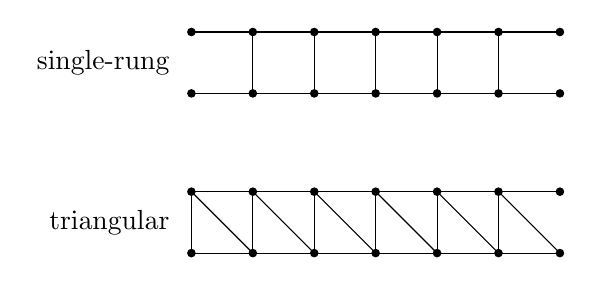
\begin{tikzpicture}[scale=0.78,>=Latex]
  \foreach \i in {0,...,6}{
    \fill (\i,2.2) circle (2pt);
    \fill (\i,1.2) circle (2pt);
  }
  \foreach \i in {0,...,5}{
    \draw (\i,2.2)--(\i+1,2.2);
    \draw (\i,1.2)--(\i+1,1.2);
  }
  \foreach \i in {1,...,5}{\draw (\i,1.2)--(\i,2.2);}
  \node[left] at (-.2,1.7) {single-rung};

  \foreach \i in {0,...,6}{
    \fill (\i,-.4) circle (2pt);
    \fill (\i,-1.4) circle (2pt);
  }
  \foreach \i in {0,...,5}{
    \draw (\i,-.4)--(\i+1,-.4);
    \draw (\i,-1.4)--(\i+1,-1.4);
    \draw (\i,-.4)--(\i,-1.4);
    \draw (\i,-.4)--(\i+1,-1.4);
  }
  \node[left] at (-.2,-.9) {triangular};
\end{tikzpicture}
\caption{The two asymptotic mechanisms.  A single rung family can force turn density $1$; two adjacent rung families form a triangular strip and yield the sharp density $2/3$.}
\end{figure}

\begin{thebibliography}{99}
\bibitem{RosalesPaperIIII}
J. Rosales P\'erez,
\emph{Unbounded Exact-Trace Confinement Gaps for Finite-Direction Lattice Spanning Paths},
preprint, 2026. DOI: 10.5281/zenodo.22065177.

\bibitem{Itai1982}
A. Itai, C. H. Papadimitriou, and J. L. Szwarcfiter,
Hamilton paths in grid graphs,
\emph{SIAM J. Comput.} 11 (1982), 676--686.

\bibitem{Arkin2005}
E. M. Arkin, M. A. Bender, E. D. Demaine, S. P. Fekete, J. S. B. Mitchell, and S. Sethia,
Optimal covering tours with turn costs,
\emph{SIAM J. Comput.} 35 (2005), 531--566.

\bibitem{FeketeKrupke2024}
S. P. Fekete and D. Krupke,
What goes around comes around: covering tours and cycle covers with turn costs,
\emph{Theory Comput. Syst.} 68 (2024), 1207--1238.

\bibitem{Fellows2009}
M. R. Fellows, P. Giannopoulos, C. Knauer, C. Paul, F. A. Rosamond, S. Whitesides, and N. Yu,
Abstract milling with turn costs,
arXiv:0912.1050.

\bibitem{Estivill2010}
V. Estivill-Castro, A. Heednacram, and F. Suraweera,
NP-completeness and FPT results for rectilinear covering problems,
\emph{J. Universal Comput. Sci.} 16 (2010), 622--652.

\bibitem{Estivill2011}
V. Estivill-Castro, A. Heednacram, and F. Suraweera,
FPT-algorithms for minimum-bends tours,
\emph{Int. J. Comput. Geom. Appl.} 21 (2011), 189--213.

\bibitem{Wang2014}
Y. Wang, X. Tan, T. Yao, J. Feng, and G. Chen,
On the minimum link-length rectilinear spanning path problem: complexity and algorithms,
\emph{IEEE Trans. Comput.} 63 (2014), 3092--3100.

\bibitem{Mitchell2014}
J. S. B. Mitchell, V. Polishchuk, and M. Sysikaski,
Minimum-link paths revisited,
\emph{Comput. Geom.} 47 (2014), 651--667.

\bibitem{Kostitsyna2017}
I. Kostitsyna, M. L\"offler, V. Polishchuk, and F. Staals,
On the complexity of minimum-link path problems,
\emph{J. Comput. Geom.} 8 (2017), 80--108.

\bibitem{Heller1957}
I. Heller,
On linear systems with integral valued solutions,
\emph{Pacific J. Math.} 7 (1957), 1351--1364.

\bibitem{OxleyWalsh2022}
J. Oxley and Z. Walsh,
2-modular matrices,
\emph{SIAM J. Discrete Math.} 36 (2022), 1231--1248.
\end{thebibliography}

\end{document}
